%% Faults and Features pages: what a fault does across sensors, and a sensor
%% across faults.
%%
%% Every figure quoted here is a macro of figures/faults/numbers.tex; the
%% tabulars are tables/faults/*.tex, each reading the CSV table beside it, and
%% the crops of the viewer are figures/faults/*.png. All are written by
%% scripts/faults.py (see README.md), from the catalogue and the files of 3W.
%% Three frames: the signature of every fault, read against the instances; the
%% same fault well by well; and what the labels of a hydrate mean.

% Written by scripts/faults.py from the catalogue and the files of 3W; do not edit by hand.
\newcommand{\faInstances}{1,119}
\newcommand{\faNormalInstances}{594}
\newcommand{\faNormalWells}{9}
\newcommand{\faScalingRise}{36}
\newcommand{\faScalingMeasured}{36}
\newcommand{\faScalingRateLow}{0.03}
\newcommand{\faScalingRateHigh}{0.70}
\newcommand{\faRestrictionInstances}{6}
\newcommand{\faRestrictionPdgLacking}{6}
\newcommand{\faRestrictionChokeLive}{1}
\newcommand{\faSluggingTpt}{2.6}
\newcommand{\faSluggingTptOver}{27}
\newcommand{\faSluggingTptOf}{32}
\newcommand{\faSluggingPdg}{0.89}
\newcommand{\faSluggingPdgOver}{4}
\newcommand{\faSluggingPdgOf}{31}
\newcommand{\faInstabilityTpt}{0.07}
\newcommand{\faHydrateReal}{14}
\newcommand{\faHydrateWells}{9}
\newcommand{\faHydrateTransientClosed}{11}
\newcommand{\faHydrateSteady}{12}
\newcommand{\faHydrateSteadyClosed}{11}
\newcommand{\faHydrateSimulated}{81}
\newcommand{\faHydrateSimulatedOpen}{100}
\newcommand{\faSimName}{SIMULATED-00001}
\newcommand{\faSimNote}{$\Delta$ = 8.38 MPa | measured 36\% (one every 2.8 s), interpolated 4\%, held 60\% | coverage 100.0 \%}
\newcommand{\faSimTicks}{1.0650,3.0650,5.0650,7.0650}
\newcommand{\faSimTickLabels}{2018-05-18 00:00,02:00,04:00,06:00}
\newcommand{\faSimLabel}{P-TPT [MPa]}
\newcommand{\faSimEnd}{7.5}
\newcommand{\faSimYmin}{19.3211}
\newcommand{\faSimYmax}{28.7120}
\newcommand{\faSimTraceColor}{1F4E79}
\newcommand{\faSimForeground}{1A1A1A}
\newcommand{\faSimNoteFill}{FFFFFF}
\newcommand{\faSimNoteBorder}{666666}
\newcommand{\faSimDotted}{1}
\newcommand{\faCaseScalingAgainst}{15}
\newcommand{\faCaseScalingOf}{19}
\newcommand{\faCaseLossAgainst}{4}
\newcommand{\faCaseLossOf}{4}
\newcommand{\faScalingRateLowWell}{WELL-00023}
\newcommand{\faScalingRateHighWell}{WELL-00001}
\newcommand{\faPressureUnit}{MPa}
\newcommand{\faCaseScalingWell}{WELL-00024}
\newcommand{\faCaseLossWell}{WELL-00016}


\newcommand{\faquestion}{\wspage{Faults \& Features pages} \raisebox{.75pt}{$\blacktriangleright$}~What does a fault do across sensors, and a sensor across faults?}

% The cells of the signature table (tables/faults/signatures.csv): the move
% the sources expect, and the instances that lack the variable.
\newcommand{\faup}{$\uparrow$}
\newcommand{\fadown}{$\downarrow$}
\newcommand{\faswing}{$\sim$}
\newcommand{\fanone}{?}
\newcommand{\fanil}{--}
\newcommand{\famiss}[1]{{\color{ws3wbrown}(#1)}}

% ---------------------------------------------------------------------------
\begin{frame}{What each fault does to its signature}
  \framesubtitle{\faquestion}
  \centering
  {%
    \scriptsize
    \setlength{\tabcolsep}{4pt}
    % Per fault class, its real instances and wells, where its signature comes
% from, and per signature variable the move the sources expect, how many
% instances make it of those that can show it, and how many instances lack the
% variable. The columns follow the placements of the viewer, topside to
% subsurface. A row is the Faults page's question, a column the Features
% page's. The cells are written by scripts/faults.py into the CSV beside this
% file; their macros are set in sections/faults.tex.
\pgfplotstabletypeset[
  columns={fault, instances, wells, source, aber_ckp, p_mon_ckp, t_jus_ckp, p_tpt, t_tpt, p_pdg},
  fa cell/.style={string type, column type={l}},
  columns/fault/.style={string type, column name={Fault}, column type={l}},
  columns/instances/.style={column name={Inst.}, column type={r}, fixed, precision=0, 1000 sep={,}},
  columns/wells/.style={column name={Wells}, column type={r}},
  columns/source/.style={string type, column name={From}, column type={l},
                         postproc cell content/.append style={/pgfplots/table/@cell content/.add={\color{ws3wbrown}}{}}},
  columns/aber_ckp/.style={fa cell, column name={ABER-CKP}},
  columns/p_mon_ckp/.style={fa cell, column name={P-MON-CKP}},
  columns/t_jus_ckp/.style={fa cell, column name={T-JUS-CKP}},
  columns/p_tpt/.style={fa cell, column name={P-TPT}},
  columns/t_tpt/.style={fa cell, column name={T-TPT}},
  columns/p_pdg/.style={fa cell, column name={P-PDG}},
  every head row/.style={
    before row={\toprule
                \multicolumn{1}{c}{\multirow{2}{*}[-1mm]{Fault}}
                & \multicolumn{3}{c}{} & \multicolumn{3}{c}{Topside}
                & \multicolumn{2}{c}{Seabed} & \multicolumn{1}{c}{Subsurface} \\
                \cmidrule(lr){5-7}\cmidrule(lr){8-9}\cmidrule(lr){10-10}},
    after row=\midrule},
  columns/fault/.append style={column name={}},
  every last row/.style={after row=\bottomrule},
]{tables/faults/signatures.csv}

    \vskip 1mm
    \begin{description}
      \item [\faup{} \fadown{}] the move the 3W paper/thesis expects from the last hour of normal operation to the last hour of the event
      \item [\faswing{}] a swing
      \item [\fanone{}] no source
      \item [\emph{a/b}] instances that make it, of those that can show it (Severe Slugging: a swing over the paper's 10\,bar). 
      \item [\famiss{m}] instances where the variable is absent or frozen
    \end{description}
  }

  \vfill
  \alert{Most signatures hold, but each has its exceptions, and some cannot be checked at all}
\end{frame}

% ---------------------------------------------------------------------------
\begin{frame}{The same fault, well by well}
  \framesubtitle{\faquestion}
  \begin{columns}[T]
    \begin{column}{0.55\textwidth}
      {\scriptsize\color{ws3wbrown} Scaling in PCK: P-MON-CKP from the onset of the transient, the
      earliest instance of each well\par}
      \vskip 1mm
      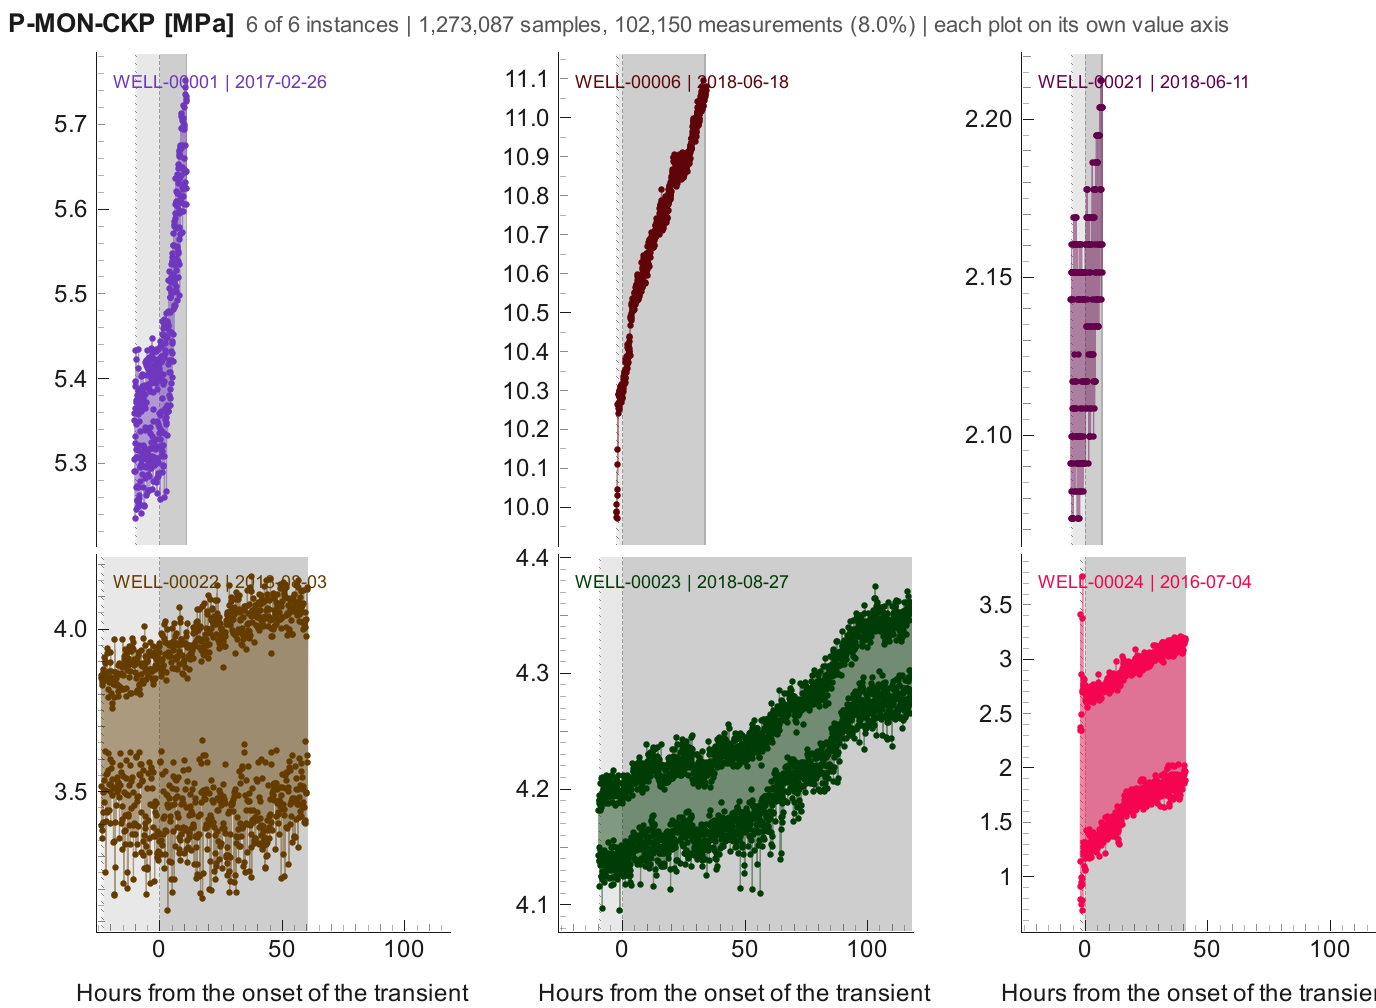
\includegraphics[width=\linewidth]{figures/faults/scaling.png}
    \end{column}
    \begin{column}{0.42\textwidth}
      \footnotesize
      \begin{itemize}
        \item \textbf{Scaling in PCK}: 
          P-MON-CKP rises in \faScalingRise{} of \faScalingMeasured{},
          but T-TPT, expected to fall, rises in \faCaseScalingAgainst{} of
          \faCaseScalingWell's \faCaseScalingOf{} instances.
      \vskip 4mm

        \item \textbf{Rapid Productivity Loss}:
          \faCaseLossWell's P-TPT rises in \faCaseLossAgainst{} of \faCaseLossOf.
      \vskip 4mm

        \item \textbf{Quick Restriction in PCK}: 
          P-PDG is frozen in \faRestrictionPdgLacking{} of
          \faRestrictionInstances{} instances, the choke opening live in \faRestrictionChokeLive.
      \vskip 4mm

        \item \textbf{Severe Slugging}: 
          swings P-TPT by \faSluggingTpt\,\faPressureUnit{}
          (median), \faSluggingTptOver{} of \faSluggingTptOf{} over 10\,bar, but P-PDG by
          \faSluggingPdg{} (\faSluggingPdgOver{} of \faSluggingPdgOf)
      \vskip 4mm
          
        \item \textbf{Flow Instability}:
          swings P-TPT by \faInstabilityTpt.
      \end{itemize}
    \end{column}
  \end{columns}
\end{frame}

% ---------------------------------------------------------------------------
\begin{frame}{Hydrate in Production Line: the ugly duckling}
  \framesubtitle{\faquestion}
  \vspace{-2mm}
  \begin{columns}[T]

    % Stacked prints of Well 19 and simulated instance; the simulated one is
    % drawn, the viewer reading only the real instances, in the crops' units.
    \begin{column}{0.5\textwidth}
      {\scriptsize\color{ws3wbrown} WELL-00019: steady means \textbf{plugged}.\par}
      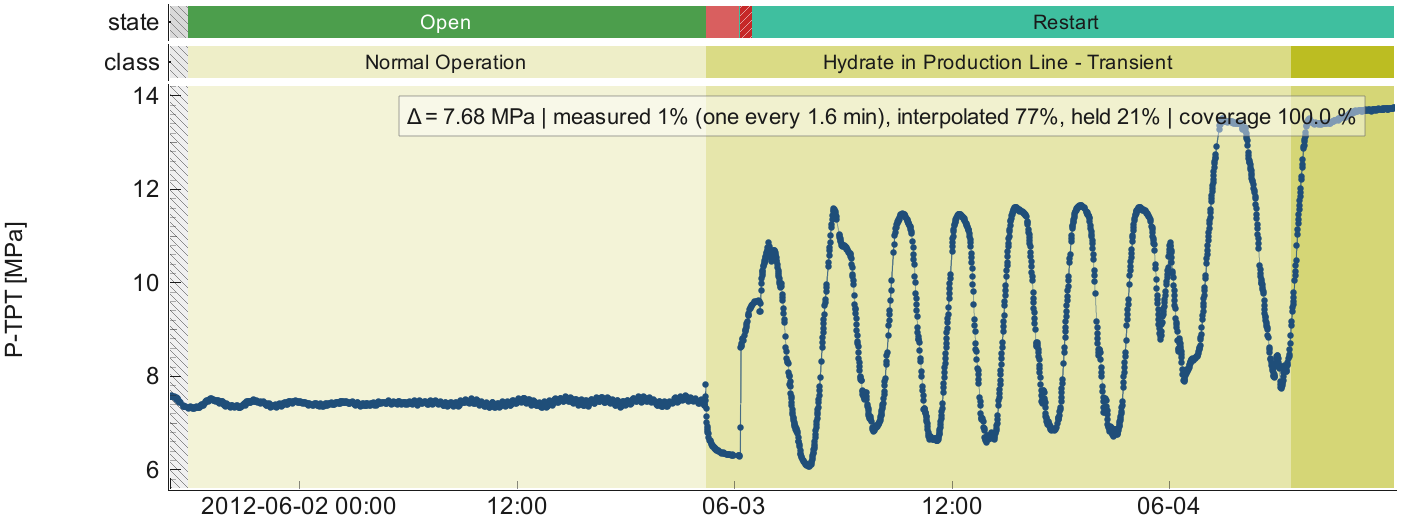
\includegraphics[width=.95\linewidth]{figures/faults/well19.png}
      %
      {\scriptsize\color{ws3wbrown} \faSimName: steady means \textbf{plugged}.\par}
      \resizebox{.95\linewidth}{!}{% A simulated hydrate as the viewer's instance window would draw it, which the
% viewer cannot, since it reads only the real instances: the state band, the
% class band, and P-TPT over the label periods shaded behind it, with the
% figures in the corner. Drawn in the window's own units, one point per pixel
% of the crops beside it (figures/faults/well19.png and well25.png, 704 by 260
% from the state band down), at the window's font sizes, so that scaled to the
% same width the three read alike: \resizebox it to the width of the crops.
%
% The data are scripts/faults.py's: the trace (simulated.csv, in hours from
% the start, the measurements flagged for the dots), the periods with the
% window's colors and names (simulated-bands.csv), and the note, the time
% ticks and the theme's colors (\faSim... in numbers.tex).
%
% Everything is inside the picture, where the ends of lines make no spaces:
% outside it, in the \resizebox, they would widen the box and shrink the plot.
\begin{tikzpicture}[font=\fontsize{11}{13}\selectfont, text=fasimfg]
  \definecolor{fasimtrace}{HTML}{\faSimTraceColor}
  \definecolor{fasimfg}{HTML}{\faSimForeground}
  \definecolor{fasimnotefill}{HTML}{\faSimNoteFill}
  \definecolor{fasimnoteborder}{HTML}{\faSimNoteBorder}
  \pgfplotstableread{figures/faults/simulated-bands.csv}\fasimbands
  \pgfplotstablegetrowsof{\fasimbands}
  \pgfmathtruncatemacro{\fasimlast}{\pgfplotsretval - 1}
  % The colors of every period, before the axis, which replays its drawing
  % later; ungrouped, so that they outlive the loop. A state has no shade.
  \pgfplotsforeachungrouped \row in {0,...,\fasimlast} {
    \pgfplotstablegetelem{\row}{fill}\of\fasimbands\edef\fasimhex{\pgfplotsretval}
    \definecolor{fasimfill\row}{HTML}{\fasimhex}
    \pgfplotstablegetelem{\row}{text}\of\fasimbands\edef\fasimhex{\pgfplotsretval}
    \definecolor{fasimtext\row}{HTML}{\fasimhex}
    \pgfplotstablegetelem{\row}{shade}\of\fasimbands\edef\fasimhex{\pgfplotsretval}
    \ifx\fasimhex\empty\else\definecolor{fasimshade\row}{HTML}{\fasimhex}\fi
    % Whether the label fits inside its span with 6 pt to spare, as the window
    % draws one only then (items.SegmentsItem); the axis is 613 pt wide. By
    % pgfmath's width(), as a picture's boxes measure nothing, in the current
    % font scaled to the band's 11 pt, as width() measures nothing either
    % once the size is changed inside it.
    \pgfplotstablegetelem{\row}{start}\of\fasimbands\let\fasimstart\pgfplotsretval
    \pgfplotstablegetelem{\row}{end}\of\fasimbands\let\fasimend\pgfplotsretval
    \pgfplotstablegetelem{\row}{label}\of\fasimbands\let\fasimlabel\pgfplotsretval
    \pgfmathsetmacro{\fasimwidth}{width("\fasimlabel") * 11 / \csname f@size\endcsname}
    \pgfmathtruncatemacro{\fasimfit}{\fasimwidth + 6 <= (\fasimend - \fasimstart) * 613 / \faSimEnd}
    \expandafter\let\csname fasimfits\row\endcsname\fasimfit
  }
  \begin{axis}[
      scale only axis, width=613pt, height=201pt,
      xmin=0, xmax=\faSimEnd, ymin=\faSimYmin, ymax=\faSimYmax,
      axis x line*=bottom, axis y line*=left, axis line style={draw=fasimfg, line width=.8pt},
      tick style={draw=fasimfg, line width=.6pt}, major tick length=5pt, minor tick length=3pt,
      tick label style={font=\fontsize{12}{14}\selectfont, text=fasimfg},
      xtick=\faSimTicks, xticklabels/.expanded=\faSimTickLabels, minor x tick num=3,
      minor y tick num=1, tick align=outside,
      ylabel=\faSimLabel,
      every axis y label/.style={at={(rel axis cs:0,0.5)}, xshift=-76pt, rotate=90,
                                 font=\fontsize{12}{14}\selectfont},
      clip=false, axis on top, set layers,
    ]
    % The label periods behind the trace, the bands above the plot.
    \pgfplotsinvokeforeach{0,...,\fasimlast}{
      \pgfplotstablegetelem{#1}{band}\of\fasimbands\let\fasimband\pgfplotsretval
      \pgfplotstablegetelem{#1}{start}\of\fasimbands\let\fasimstart\pgfplotsretval
      \pgfplotstablegetelem{#1}{end}\of\fasimbands\let\fasimend\pgfplotsretval
      \pgfplotstablegetelem{#1}{label}\of\fasimbands\let\fasimlabel\pgfplotsretval
      \def\fasimclass{class}
      % The class band sits 4 pt over the plot, the state band 4 pt over that.
      \ifx\fasimband\fasimclass
        \def\fasimrise{4pt}
        \edef\fasimdraw{\noexpand\fill [fasimshade#1]
          (axis cs:\fasimstart,\faSimYmin) rectangle (axis cs:\fasimend,\faSimYmax);}
        \fasimdraw
      \else
        \def\fasimrise{24pt}
      \fi
      % The label only where it fits (measured above).
      \ifnum\csname fasimfits#1\endcsname=1
        \edef\fasimnode{node [midway, text=fasimtext#1] {\fasimlabel}}
      \else
        \def\fasimnode{}
      \fi
      \edef\fasimdraw{\noexpand\fill [fasimfill#1]
        ([yshift=\fasimrise]axis cs:\fasimstart,\faSimYmax)
        rectangle ([yshift=\fasimrise+16pt]axis cs:\fasimend,\faSimYmax) \fasimnode;}
      \fasimdraw
    }
    \node [anchor=east, font=\fontsize{12}{14}\selectfont] at ([xshift=-8pt, yshift=12pt]rel axis cs:0,1) {class};
    \node [anchor=east, font=\fontsize{12}{14}\selectfont] at ([xshift=-8pt, yshift=32pt]rel axis cs:0,1) {state};
    % The trace: the line faint between measurements, dots on them, where the
    % window would dot the series at all.
    \ifnum\faSimDotted=1
      \addplot [fasimtrace, line width=1pt, draw opacity=.45, no marks]
        table [x=hours, y=value] {figures/faults/simulated.csv};
      \addplot [only marks, mark=*, mark size=1.6pt, mark options={draw=none, fill=fasimtrace}]
        table [x=hours, y=value, restrict expr to domain={\thisrow{measured}}{1:1}]
        {figures/faults/simulated.csv};
    \else
      \addplot [fasimtrace, line width=1pt, no marks] table [x=hours, y=value]
        {figures/faults/simulated.csv};
    \fi
    % The figures in the corner, on a see-through box over the trace, as the
    % window lays it: on the foreground layer, the plots being drawn last.
    \begin{pgfonlayer}{axis foreground}
      \node [anchor=south east, draw=fasimnoteborder, line width=.6pt, fill=fasimnotefill,
             fill opacity=.43, text opacity=1, inner xsep=5pt, inner ysep=3pt,
             font=\fontsize{10.5}{12}\selectfont]
        at ([xshift=-14pt, yshift=5pt]rel axis cs:1,0) {\faSimNote};
    \end{pgfonlayer}
    \coordinate (fasim-sw) at (rel axis cs:0,0);
    \coordinate (fasim-ne) at (rel axis cs:1,1);
  \end{axis}
  % The crops' frame: 84 pt of labels on the left, 7 on the right, the bands
  % and their gaps above (43 pt), the time ticks below (16 pt).
  \pgfresetboundingbox
  \path [use as bounding box]
    ([xshift=-84pt, yshift=-16pt]fasim-sw) rectangle ([xshift=7pt, yshift=43pt]fasim-ne);
\end{tikzpicture}
}
    \end{column}

    % Bullet points
    \begin{column}{.5\textwidth}
      {\scriptsize\color{ws3wbrown} WELL-00025: steady means \textbf{reopened}.\par}
      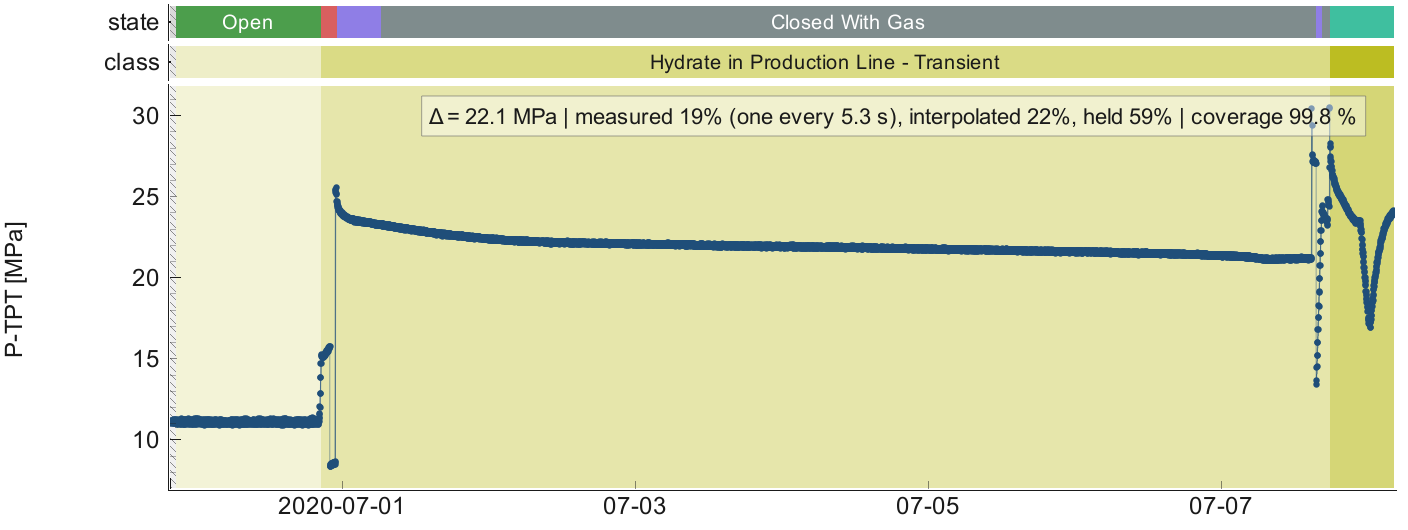
\includegraphics[width=.95\linewidth]{figures/faults/well25.png}
      
      % Summary
      \vskip 10mm
      \centering
      \alert{Hydrate labeling across instances, real or simulated, do not seem to share the same philosophy}
      \vskip 2mm
      \hyperlink{hydrate labels}{\beamergotobutton{Appendix}}
    \end{column}
  \end{columns}
\end{frame}
